\section{支持向量机}

\subsection{逻辑回归的缺陷}
\begin{enumerate}
	\item 按照逻辑回归的计算方式,我们得到的是一个分隔线(或平面或超平面\footnote{1维称为线,2维称为平面,更多维就称为超平面}),对于我们的数据点,总有一些点离超平面较近(如点C),有一些点离超平面较远(如点A);对于离超平面较远的点,我们有很大把握保证我们的预测是准确的,但是,对于离超平面较近的点我们就没把握了。
	\begin{figure}[htbp]
		\centering
		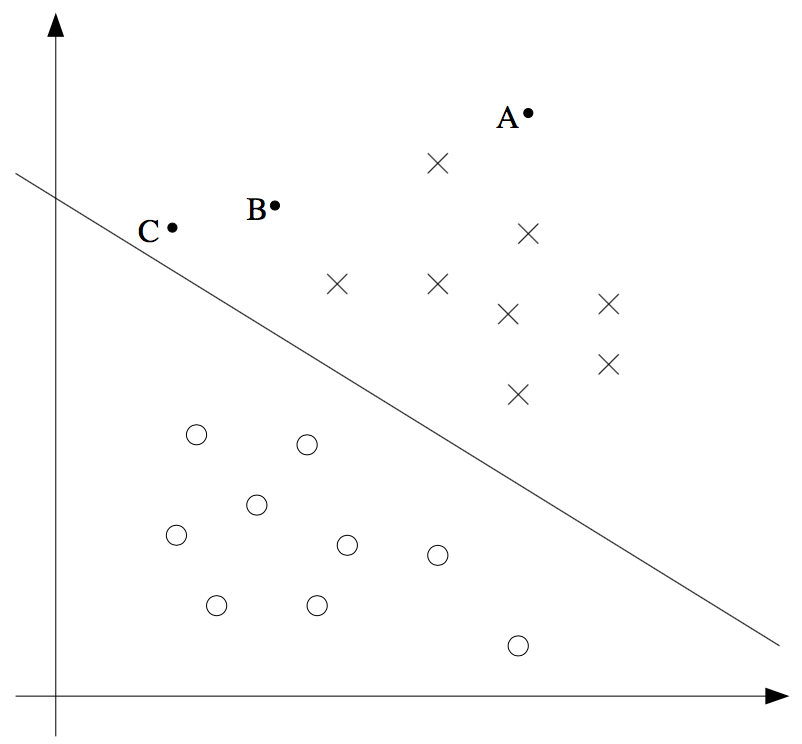
\includegraphics[scale=0.5]{images/逻辑回归缺陷讲述}
	\end{figure}
\end{enumerate}

\subsection{SVM前言}
\begin{enumerate}
	\item 在后续介绍SVM过程中,为了描述方便,我们对之前逻辑回归的一些描述做了更改
	\item 将$y \& h$的值从值域$\{0,1\}$切换到$\{-1, 1\}$,其中,$0\to -1$,$1\to 1$
	\item 将$h_\theta(x)$更改为$h_{w,b}(x)$,其中:$w \to \left[\begin{matrix}\theta_1 \\ \theta_2 \\ \vdots \\ \theta_n  \end{matrix}\right]$,$b \to \theta_0$\footnote{此处为了表达方便,使用$\to$来表达类似的对应关系,且勿将其当做等于"$=$"},且取消原有的$x_0=1$假设。通过此方式将$h(x)$由参数$\theta$变成了参数$w, b$,将截距项$b$与其他项分隔开,以便分析
\end{enumerate}

\subsection{Margin介绍}
\subsubsection{函数间隔}
\begin{enumerate}
	\item 对于数据点$(x^{(i)}, y^{(i)})$,其函数间隔定义为:
	\begin{align}
		\hat{\gamma}^{(i)} = y^{(i)}(w^Tx^{(i)} + b)
	\end{align}
	\item 对于$y^{(i)}=1$的点,为了让函数间隔$\hat{\gamma}$越大,我们需要让$w^Tx^{(i)} + b$正向越大;
	\item 对于$y^{(i)}=-1$的点,为了让函数间隔$\hat{\gamma}$越大,我们需要让$w^Tx^{(i)} + b$负向越大;
	\item 对于给定的训练集$S=\{(x^{(i)}, y^{(i)}); \quad i = 1, \dots, m\}$,我们将其中最小的函数间隔记为$\hat{\gamma}$:
	\begin{align}
		\hat{\gamma} = \min_{i=1,\dots,m}\hat{\gamma}^{(i)}
	\end{align}
	\item 对于函数间隔,若将参数$(w,b)$扩大2倍2为$(2w,2b)$,函数间隔的值$\hat{h}_{w,b}(x)$也变成了原来的2倍,但实际上,这对训练的效果并没有影响,原来错误的现在还是错误
\end{enumerate}

\subsubsection{几何间隔}
\begin{enumerate}
	\item 几何间隔表示为$\gamma^{(i)}$\footnote{与函数间隔相比,少了头顶的帽子: $\hat{ }$}。
	\item 对于数据点$(x^{(i)}, y^{(i)})$,其几何间隔定义为\footnote{证明过程略}:
	\begin{align}
		\gamma^{(i)} &= \frac{\hat{\gamma}^{(i)}}{\|w\|}  \\
		&= \frac{y^{(i)}(w^Tx^{(i)} + b)}{\|w\|}  \\
		&=  y^{(i)} \left(\left(\frac{w}{\|w\|}\right)^T x^{(i)} + \frac{b}{\|w\|}\right)
	\end{align}
	\item 当$\|w\|=1$时,几何间隔与函数间隔相等
	\item 相较于函数间隔,几何间隔任意缩放参数$(w,b)$不影响$h_{w,b}(x)$的值;鉴于此性质,我们可以在训练时对$w, b$视需求进行缩放
	\item 同样,对于给定的训练集$S=\{(x^{(i)}, y^{(i)}); \quad i = 1, \dots, m\}$,我们将其中最小的几何间隔记为$\gamma$:
	\begin{align}
		\gamma = \min_{i=1,\dots,m}\gamma^{(i)}
	\end{align}
\end{enumerate}
























